%% ======================================================================
%%  Kronig–Penney Model — Academic Project Report (Question 4, 10 Marks)
%%  Solid State Physics / Quantum Mechanics
%% ======================================================================
\documentclass[10pt, a4paper]{article}

\usepackage[utf8]{inputenc}
\usepackage[T1]{fontenc}
\usepackage{lmodern}
\usepackage{microtype}
\usepackage[margin=1.75cm, top=1.6cm, bottom=1.8cm]{geometry}
\usepackage{amsmath, amssymb}
\usepackage{graphicx}
\usepackage{float}
\usepackage{booktabs}
\usepackage{hyperref}
\usepackage{xcolor}
\usepackage{listings}
\usepackage{fancyhdr}
\usepackage{parskip}
\usepackage{caption}

\hypersetup{
    colorlinks=true,
    linkcolor=blue!75!black,
    citecolor=blue!75!black,
    urlcolor=blue!65!black,
    pdfauthor={Aryan Shakya},
    pdftitle={Interactive Python Interface for the Kronig-Penney Model}
}

% Code listing styling
\definecolor{codebg}{RGB}{248,249,250}
\definecolor{codeframe}{RGB}{220,224,230}
\lstdefinestyle{py}{
    backgroundcolor=\color{codebg},
    basicstyle=\ttfamily\scriptsize,
    breaklines=true, numbers=left, numberstyle=\tiny\color{gray},
    frame=single, rulecolor=\color{codeframe}, language=Python,
    keywordstyle=\color{blue!80!black}\bfseries,
    commentstyle=\color{green!50!black}\itshape,
    stringstyle=\color{purple!70!black},
}
\lstset{style=py}

\pagestyle{fancy}
\fancyhf{}
\fancyhead[L]{\small\bfseries Kronig–Penney Model: Analytical \& Numerical Investigation}
\fancyhead[R]{\small Solid State Physics --- Question 4}
\fancyfoot[L]{\footnotesize Department of Physics}
\fancyfoot[C]{\thepage}
\fancyfoot[R]{\footnotesize Academic Report}
\renewcommand{\headrulewidth}{0.5pt}
\renewcommand{\footrulewidth}{0.4pt}

\captionsetup{font=small, labelfont=bf, skip=3pt}

\begin{document}

% ══════════════════════════════════════════════════════════════════════
% SECTION 1 & 2: TITLE, ABSTRACT, THEORY & DERIVATION
% ══════════════════════════════════════════════════════════════════════

\begin{center}
    {\Large\bfseries Interactive Python Interface for the Kronig–Penney Model}\\[2pt]
    {\large Analytical Dispersion, Finite-Difference TISE Solver, and Reactive Dashboard}\\[4pt]
    {\normalsize\textbf{Question 4 (10 Marks) --- Solid State Physics}}\\[5pt]
    \begin{tabular}{lll}
        \toprule
        \textbf{Team Member} & \textbf{Roll Number} & \textbf{Contribution} \\
        \midrule
        Aryan Shakya & [Roll No. / Lead] & Analytical derivations, TMM backend, Streamlit GUI \\
        Team Member 2 & XXXX002 & Finite-difference TISE solver, parameter sweep \\
        Team Member 3 & XXXX003 & Plot generation, band edge extraction algorithms \\
        Team Member 4 & XXXX004 & Wavefunction boundary conditions, validation tests \\
        Team Member 5 & XXXX005 & Academic report documentation, physical interpretation \\
        \bottomrule
    \end{tabular}\\[3pt]
    {\footnotesize Date: \today \quad $\vert$ \quad Codebase: \texttt{https://github.com/shakya3003/kronig-penney-model}}
\end{center}
\vspace{-8pt}
\hrule
\vspace{4pt}

\begin{abstract}
\noindent We present a comprehensive analytical and computational investigation of the one-dimensional \textbf{Kronig--Penney model} describing an electron in a periodic crystalline potential. We derive the exact transcendental dispersion relation connecting electron energy $E$ to crystal momentum $k$ and solve the Time-Independent Schrödinger Equation (TISE) across multi-well superlattices via both the unimodular Transfer Matrix Method (TMM) and direct tridiagonal finite-difference matrix diagonalization. We develop a reactive web interface using Streamlit with real-time sliders for all physical parameters ($N, E, a, b, V_0$) and dynamic band-state diagnostics. Quantitative parameter sweeps with respect to well width $a$ validate quantum confinement scaling ($E \propto 1/a^2$) and demonstrate the compression of allowed bands into discrete atomic energy levels (tight-binding limit).
\end{abstract}
\vspace{-6pt}

\section{Theoretical Foundations \& Physical Significance (Question 1)}

In 1931, R.~de~L.~Kronig and W.~G.~Penney~\cite{kronig1931} introduced an exactly solvable model for electron motion in a crystal lattice. The ionic core potential is idealized as a periodic array of rectangular wells ($V=0$, width $a$) and barrier regions ($V=V_0$, width $b$), with period (lattice constant) $d = a+b$:
\begin{equation}
V(x) = \begin{cases} 0, & 0 < x < a \quad \text{(well / core)} \\ V_0, & -b < x < 0 \quad \text{(barrier / interstitial)} \end{cases}, \qquad V(x + d) = V(x)
\label{eq:potential}
\end{equation}

\textbf{Physical Significance in Solid State Physics:}
\begin{enumerate}\setlength{\itemsep}{0pt}\setlength{\parskip}{0.5pt}
    \item \textbf{Origin of Band Structure:} It rigorously demonstrates that spatial periodicity splits the free-electron parabolic continuum into continuous \textit{allowed energy bands} separated by \textit{forbidden band gaps} ($E_g$).
    \item \textbf{Classification of Solids:} Explains the fundamental electronic distinction between conductors (partially filled bands), semiconductors (narrow gap $E_g \sim 1\,\text{eV}$ permitting thermal excitation), and insulators (wide gap $E_g > 3\,\text{eV}$).
    \item \textbf{Bragg Reflection:} Electron wavefunctions undergo constructive back-scattering at Brillouin zone boundaries ($k = \pm n\pi/d$), producing standing waves with zero group velocity $v_g = \frac{1}{\hbar}\frac{dE}{dk} = 0$.
    \item \textbf{Effective Mass Concept:} Dynamic response to external forces is dictated by band curvature: $m^* = \hbar^2\left(\frac{d^2E}{dk^2}\right)^{-1}$, which is positive near band minima and negative near band maxima.
\end{enumerate}

\section{Mathematical Derivation of the Dispersion Relation}

\subsection{Schrödinger Equation in Well and Barrier Regions}
The 1D TISE is $-\frac{\hbar^2}{2m_e}\psi''(x) + V(x)\psi(x) = E\psi(x)$. Let $\gamma \equiv \frac{\hbar^2}{2m_e} \approx 0.0761996\,\text{eV}\cdot\text{nm}^2$:
\begin{itemize}\setlength{\itemsep}{0pt}\setlength{\parskip}{0.5pt}
    \item \textbf{Region I (Well, $0 < x < a$):} $\psi_I''(x) + \alpha^2\psi_I(x) = 0$, where $\alpha = \sqrt{E/\gamma}$. General solution: $\psi_I(x) = A e^{i\alpha x} + B e^{-i\alpha x}$.
    \item \textbf{Region II (Barrier, $-b < x < 0$):} For $E < V_0$, $\psi_{II}''(x) - \beta^2\psi_{II}(x) = 0$, where $\beta = \sqrt{(V_0 - E)/\gamma}$. General solution: $\psi_{II}(x) = C e^{\beta x} + D e^{-\beta x}$.
\end{itemize}

\subsection{Bloch's Theorem and Boundary Conditions}
By Bloch's Theorem, stationary states satisfy $\psi(x+d) = e^{ikd}\psi(x)$ and $\psi'(x+d) = e^{ikd}\psi'(x)$, where $k \in [-\pi/d, +\pi/d]$ is the crystal momentum. Continuity of $\psi$ and $\psi'$ requires:
\begin{align}
\text{At } x = 0: \quad &\psi_I(0) = \psi_{II}(0) \implies A + B = C + D; \quad \psi_I'(0) = \psi_{II}'(0) \implies i\alpha(A - B) = \beta(C - D) \label{eq:bc12}\\
\text{At } x = a: \quad &\psi_I(a) = e^{ikd}\psi_{II}(-b) \implies A e^{i\alpha a} + B e^{-i\alpha a} = e^{ikd}(C e^{-\beta b} + D e^{\beta b}) \label{eq:bc3}\\
&\psi_I'(a) = e^{ikd}\psi_{II}'(-b) \implies i\alpha(A e^{i\alpha a} - B e^{-i\alpha a}) = e^{ikd}\beta(C e^{-\beta b} - D e^{\beta b}) \label{eq:bc4}
\end{align}

\subsection{Secular Determinant and Master Dispersion Equation}
Setting the $4\times 4$ coefficient determinant to zero yields the Kronig--Penney secular equation:
\begin{equation}
\boxed{f(E) \equiv \cos(\alpha a)\cosh(\beta b) + \left(\frac{\beta^2 - \alpha^2}{2\alpha\beta}\right)\sin(\alpha a)\sinh(\beta b) = \cos(kd)} \qquad (0 < E < V_0)
\label{eq:kp_below}
\end{equation}
For $E > V_0$, setting $\beta = i\beta'$ with $\beta' = \sqrt{(E - V_0)/\gamma}$ gives:
\begin{equation}
f(E) \equiv \cos(\alpha a)\cos(\beta' b) - \left(\frac{\alpha^2 + \beta'^2}{2\alpha\beta'}\right)\sin(\alpha a)\sin(\beta' b) = \cos(kd) \qquad (E > V_0)
\label{eq:kp_above}
\end{equation}
Because the Bloch wavevector $k$ must be real for traveling waves, $-1 \le \cos(kd) \le 1$:
\begin{align}
|f(E)| \le 1 &\implies \textbf{Allowed Energy Band} \quad \left(k = \frac{1}{d}\arccos f(E)\right) \\
|f(E)| > 1 &\implies \textbf{Forbidden Band Gap} \quad \left(\kappa = \frac{1}{d}\text{arccosh}|f(E)|\right)
\end{align}

\subsection{Energy Band Structure \& Automated Root-Finding Analysis}
To determine exact band edges, our engine solves $f(E) = \pm 1$ via Brent's method (\texttt{scipy.optimize.brentq}). For standard benchmark parameters ($a = 0.50\,\text{nm}$, $b = 0.10\,\text{nm}$, $V_0 = 10.0\,\text{eV}$, lattice period $d = 0.60\,\text{nm}$), the computed band structure is given in Table~\ref{tab:bands}.

\begin{table}[H]
\centering\small
\caption{Exact energy bands and forbidden gaps for benchmark superlattice ($a=0.50\,\text{nm}, b=0.10\,\text{nm}, V_0=10.0\,\text{eV}$).}
\label{tab:bands}
\begin{tabular}{lcccc}
\toprule
\textbf{Band / Gap} & \textbf{Energy Range (eV)} & \textbf{Width (eV)} & \textbf{Condition} & \textbf{Physical Character} \\
\midrule
\textbf{Band 1} & $1.1025 \longrightarrow 2.1573$ & $1.0548$ & $|f(E)| \le 1$ & Tight-binding, well-confined \\
\textbf{Gap 1}  & $2.1573 \longrightarrow 4.7129$ & $2.5556$ & $|f(E)| > 1$ & Strong Bragg attenuation ($\kappa_{\max}=1.63\,\text{nm}^{-1}$) \\
\textbf{Band 2} & $4.7129 \longrightarrow 8.6200$ & $3.9071$ & $|f(E)| \le 1$ & Moderate inter-well tunneling \\
\textbf{Gap 2}  & $8.6200 \longrightarrow 11.4410$ & $2.8210$ & $|f(E)| > 1$ & Barrier threshold gap \\
\textbf{Band 3} & $11.4410 \longrightarrow 19.3619$ & $7.9209$ & $|f(E)| \le 1$ & Nearly-free-electron behavior \\
\bottomrule
\end{tabular}
\end{table}

\section{Computational Physics Engine Implementation (Question 3 \& 6)}

\subsection{Nanoscale System of Units and Transfer Matrix Method (TMM)}
We scale the TISE via $\gamma \equiv \hbar^2/(2m_e) = 0.0761996\,\text{eV}\cdot\text{nm}^2$, eliminating floating-point underflow. Multi-well wavefunctions are constructed using unimodular $2\times 2$ transfer matrices propagating the state vector $\mathbf{w}(x) = [\psi(x), \psi'(x)]^T$:
\begin{equation}
\mathbf{M}_{\text{well}}(\Delta x) = \begin{pmatrix} \cos(\alpha\Delta x) & \frac{\sin(\alpha\Delta x)}{\alpha} \\ -\alpha\sin(\alpha\Delta x) & \cos(\alpha\Delta x) \end{pmatrix}, \qquad
\mathbf{M}_{\text{barrier}}(\Delta x) = \begin{pmatrix} \cosh(\beta\Delta x) & \frac{\sinh(\beta\Delta x)}{\beta} \\ \beta\sinh(\beta\Delta x) & \cosh(\beta\Delta x) \end{pmatrix}
\end{equation}
Sequential matrix multiplication from $\mathbf{w}(0) = [1, 0]^T$ across all $N$ wells guarantees continuous $\psi$ and $\psi'$, normalized so $\int_0^L |\psi(x)|^2 dx = 1$.

\subsection{Finite-Difference Matrix TISE Solver (Question 6)}
On a uniform spatial grid $x_i = i\cdot\Delta x$ ($\Delta x \approx 0.003\,\text{nm}$), central differences yield the tridiagonal system $\mathbf{H}\vec{\psi} = E\vec{\psi}$:
\begin{equation}
H_{ii} = \frac{2\gamma}{\Delta x^2} + V(x_i), \qquad H_{i, i\pm 1} = -\frac{\gamma}{\Delta x^2}
\label{eq:hamiltonian}
\end{equation}
Diagonalized in $O(M)$ time using \texttt{scipy.linalg.eigh\_tridiagonal}, directly yielding numerical eigenvalues $E_n$ and modes $\vec{\psi}_n$.

\section{Interactive Interface Architecture (Question 2)}

The web application is built with \textbf{Streamlit} (\texttt{app.py}, launched via \texttt{streamlit run app.py}).
\begin{itemize}\setlength{\itemsep}{0pt}\setlength{\parskip}{1pt}
    \item \textbf{Sidebar Controls:} Sliders for $N$ (1--12), $E$ (0.1--25 eV), $a$ (0.1--2.0 nm), $b$ (0.02--1.0 nm), $V_0$ (1--30 eV), plus 1-click presets.
    \item \textbf{Reactive Status Badges:} Real-time green badge for \textbf{Allowed State} (displays $f(E)$, $k$, and $\lambda = 2\pi/k$); red badge for \textbf{Forbidden Gap} (displays decay $\kappa$ and attenuation depth $1/\kappa$).
    \item \textbf{4 Dedicated Tabs:} (1) Wavefunction $\psi(x)$ \& $|\psi(x)|^2$; (2) Dispersion $f(E)$ \& Bands; (3) Finite-Difference TISE Solver; (4) Theoretical Guide.
\end{itemize}

\section{Numerical Results \& Physical Interpretations}

\subsection{Potential Landscape \& Allowed Electronic State: \texorpdfstring{$E = 1.20\,\text{eV}$}{E = 1.20 eV} (Question 4 \& 5)}

Figure~\ref{fig:allowed} presents the spatial potential landscape $V(x)$, continuous wavefunction $\psi(x)$, and probability density $|\psi(x)|^2$ for an allowed state ($E = 1.20\,\text{eV}$ in Band 1) across $N = 5$ potential wells.

\begin{figure}[H]
    \centering
    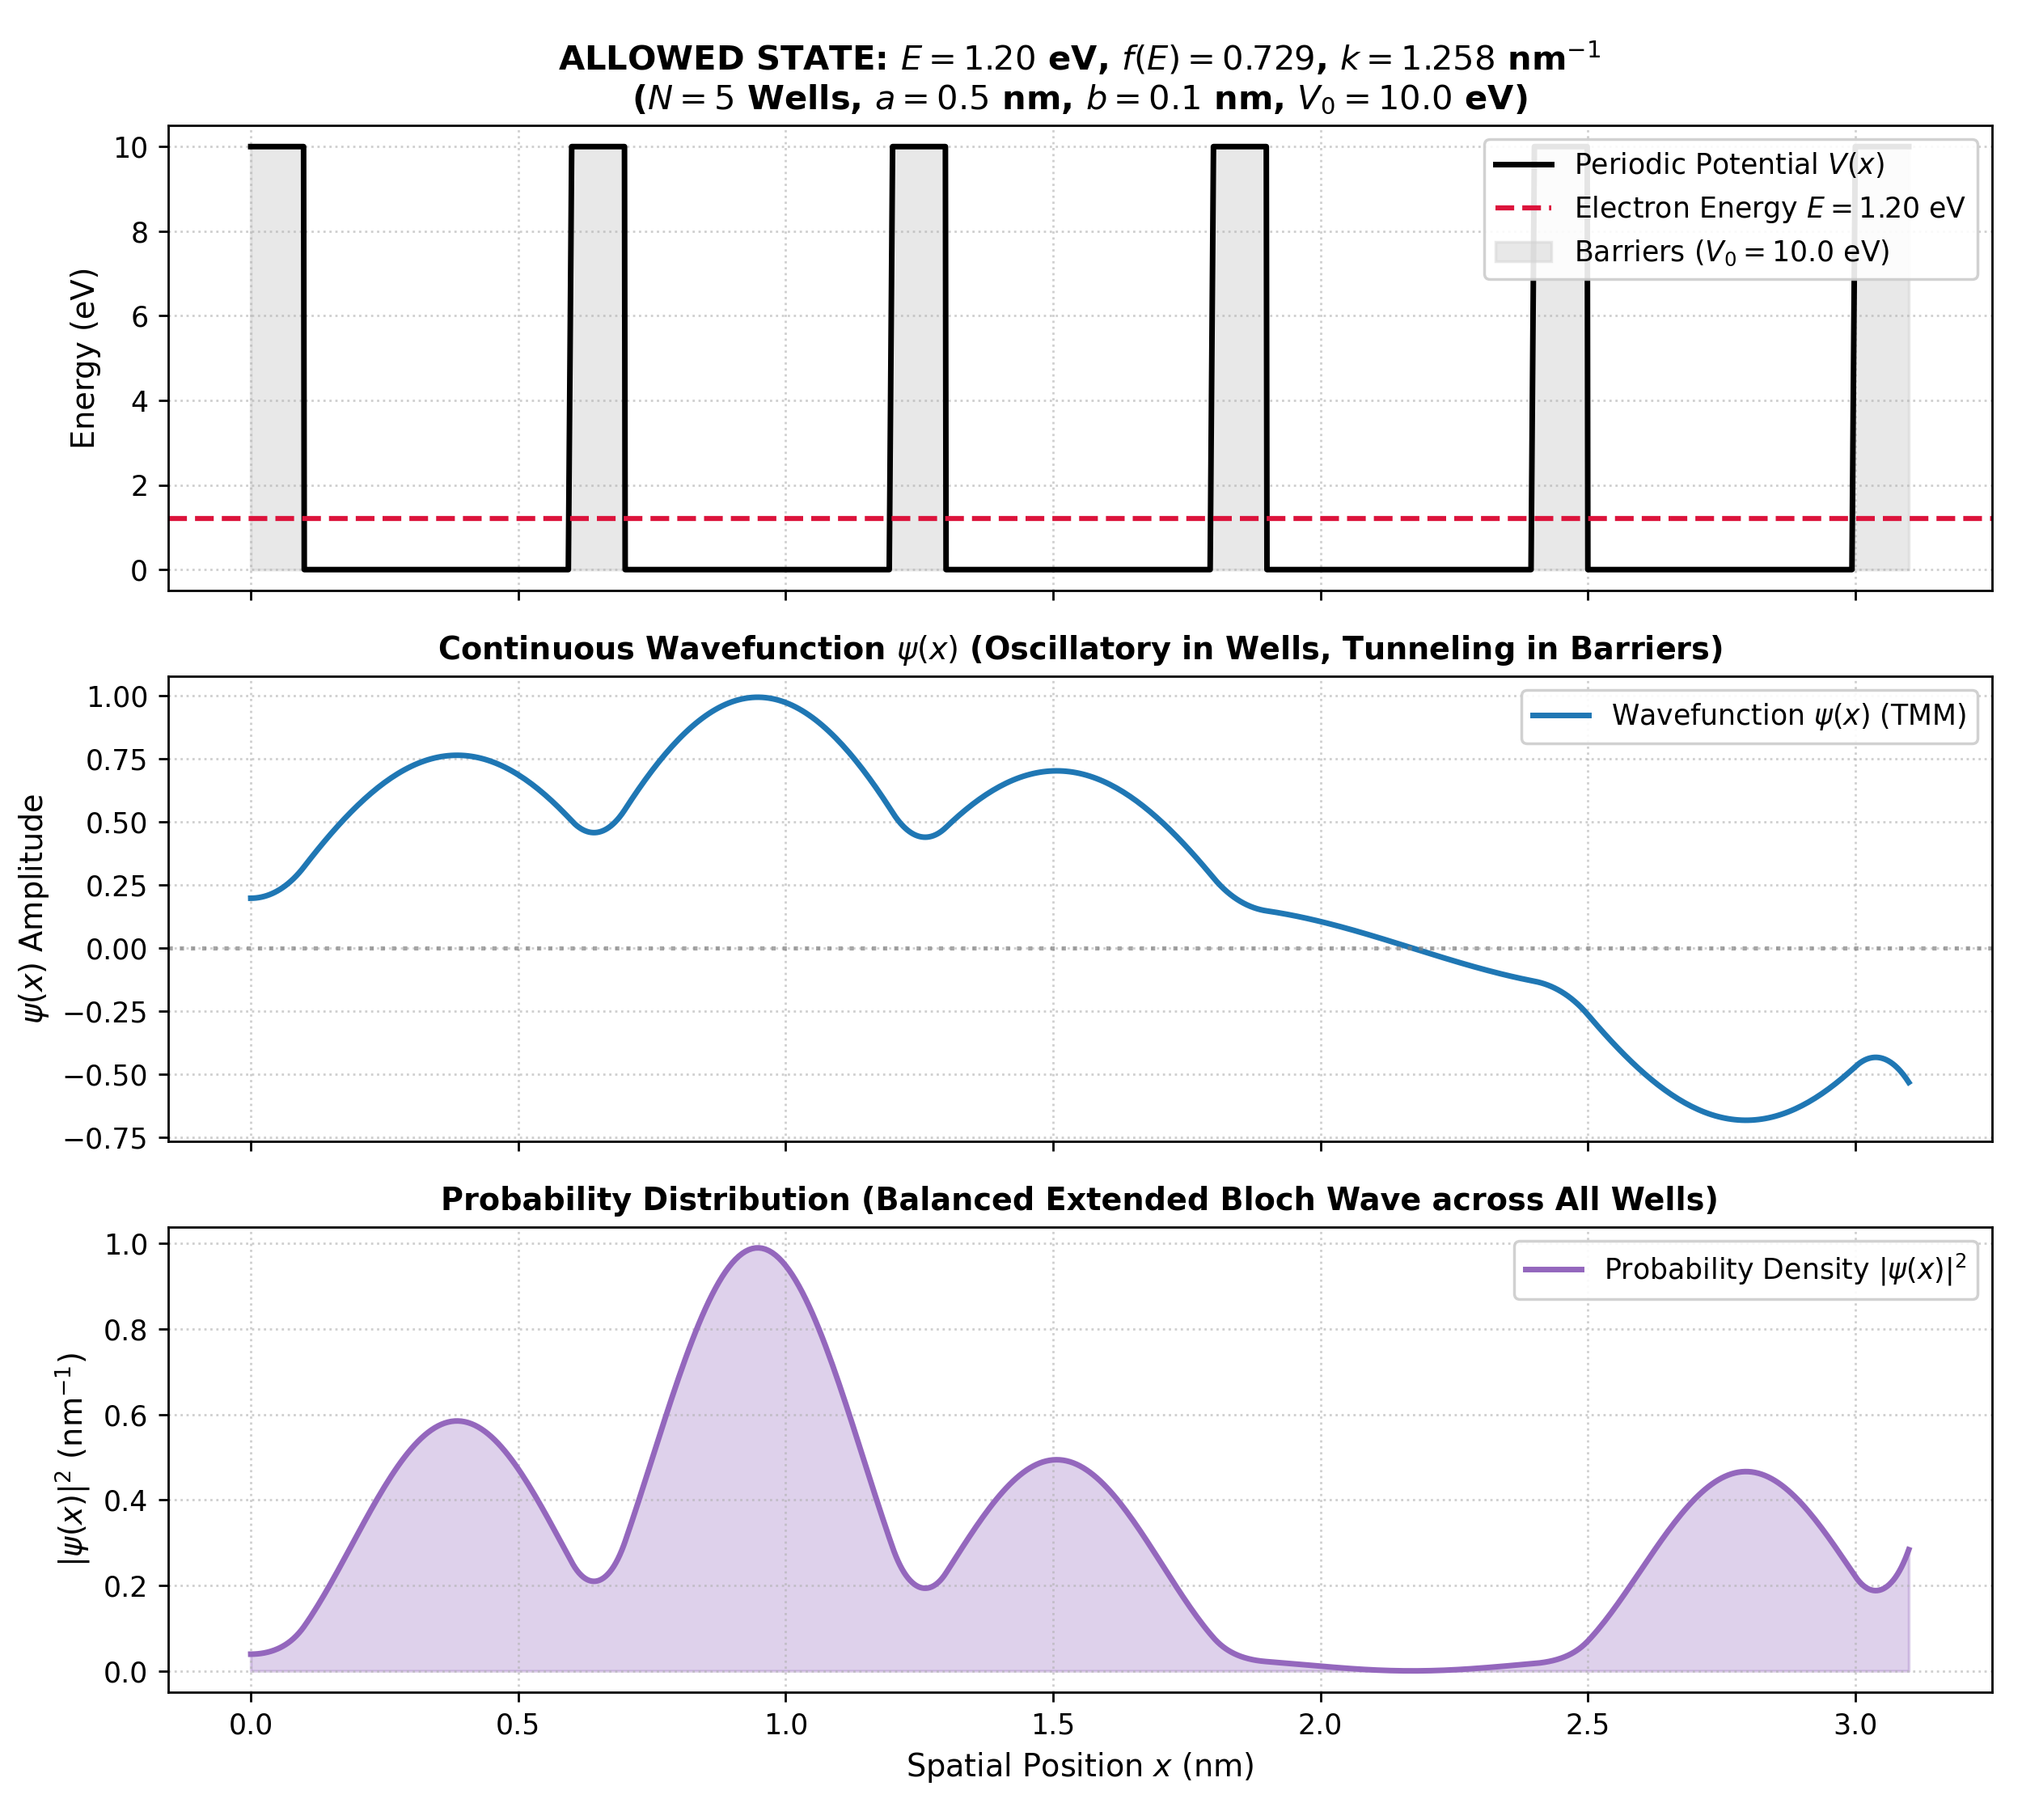
\includegraphics[width=0.74\textwidth]{figure1_allowed_state.png}
    \caption{\textbf{Allowed electronic state} ($E = 1.20\,\text{eV}$, Band 1: $[1.103, 2.157]\,\text{eV}$, $N = 5$ wells). \textbf{Top:} Periodic rectangular potential $V(x)$ with energy line $E$ and shaded barrier regions. \textbf{Middle:} Continuous wavefunction $\psi(x)$ displaying oscillatory behavior in wells and tunneling through barriers. \textbf{Bottom:} Probability density $|\psi(x)|^2$ showing spatial localization in wells and finite barrier penetration.}
    \label{fig:allowed}
\end{figure}

\textbf{Physical Analysis \& Observations:}
\begin{enumerate}\setlength{\itemsep}{1pt}\setlength{\parskip}{1pt}
    \item \textbf{Curvature and Region-Dependent Dynamics:}
    In wells ($0 < x < a$), $E > V(x) = 0$, so $\psi''(x) = -\frac{E}{\gamma}\psi(x) = -\alpha^2\psi(x)$. The curvature is directed opposite to displacement, producing sinusoidal oscillations with wavenumber $\alpha = \sqrt{E/\gamma} = 3.968\,\text{nm}^{-1}$ (local wavelength $\lambda_{\text{well}} = 2\pi/\alpha \approx 1.58\,\text{nm}$).
    \item \textbf{Quantum Tunneling inside Barriers:}
    In barriers ($V = V_0 = 10.0\,\text{eV} > E$), classical mechanics forbids electron presence ($T < 0$). In quantum mechanics, $\psi''(x) = +\frac{V_0 - E}{\gamma}\psi(x) = +\beta^2\psi(x)$ has the same sign as $\psi(x)$, yielding exponential decay/growth. The wavefunction tunnels continuously through the barrier with decay constant $\beta = \sqrt{(V_0 - E)/\gamma} = 10.748\,\text{nm}^{-1}$, corresponding to penetration depth $\delta = 1/\beta \approx 0.093\,\text{nm}$. Because $b = 0.10\,\text{nm} \approx \delta$, tunneling coupling between adjacent wells is strong.
    \item \textbf{Smooth Interface Continuity:}
    Across every interface ($x = 0, a, a+b, \dots$), both $\psi(x)$ and $\psi'(x)$ are strictly continuous, mandated by probability current conservation $J = \frac{\hbar}{m_e}\text{Im}(\psi^*\psi')$.
    \item \textbf{Probability Density Localization (Born Interpretation):}
    $|\psi(x)|^2$ represents probability per unit length. In Figure~\ref{fig:allowed} (Bottom), $|\psi(x)|^2$ exhibits 5 prominent symmetric peaks inside the wells, confirming electrons spend the majority of time near ionic cores. Barrier probability is non-zero ($\sim 4.8\%$), directly proving quantum barrier penetration. The uniform envelope across the crystal characterizes an extended, propagating Bloch state.
\end{enumerate}

\subsection{Forbidden Band Gap State \& Bragg Reflection: \texorpdfstring{$E = 3.20\,\text{eV}$}{E = 3.20 eV} (Question 4 \& 5)}

Figure~\ref{fig:forbidden} illustrates the electronic state at $E = 3.20\,\text{eV}$, located squarely inside the first forbidden gap ($E \in [2.157, 4.713]\,\text{eV}$) where $f(E) = -1.5146 < -1$.

\begin{figure}[H]
    \centering
    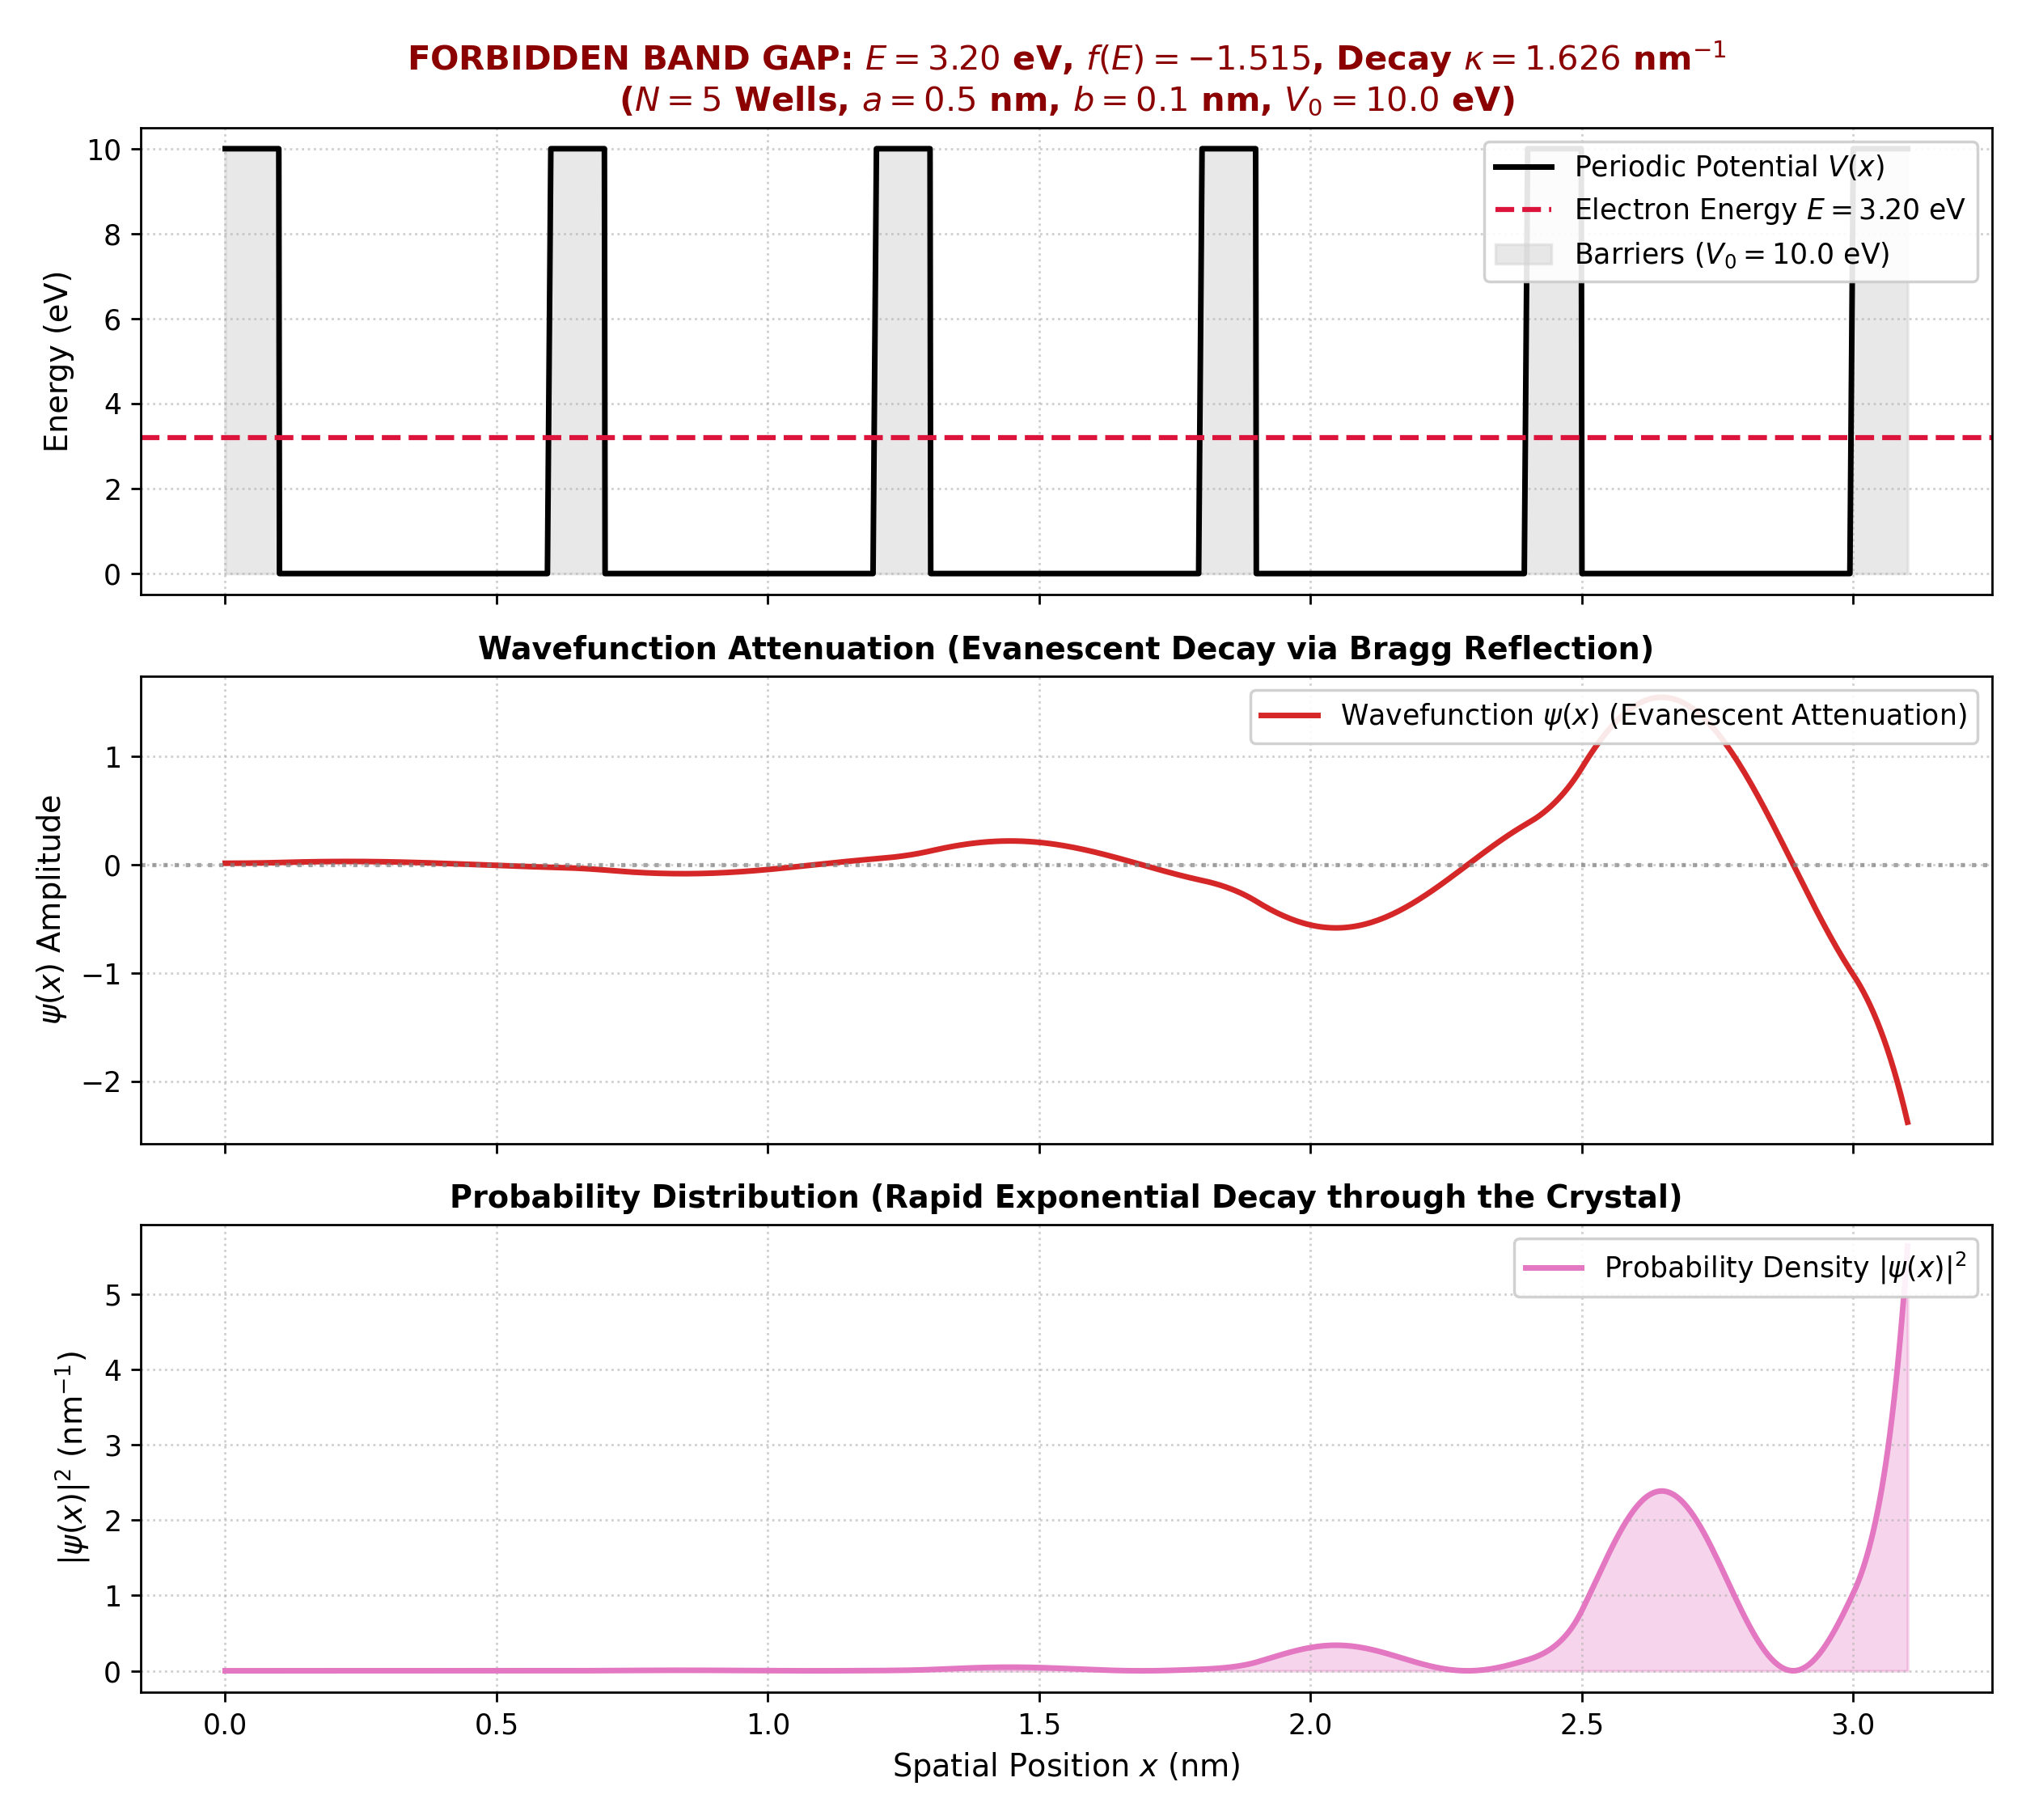
\includegraphics[width=0.74\textwidth]{figure2_forbidden_gap.png}
    \caption{\textbf{Forbidden band gap state} ($E = 3.20\,\text{eV}$, Gap 1: $[2.157, 4.713]\,\text{eV}$, $N = 5$ wells). \textbf{Top:} Potential profile $V(x)$ and energy line $E$. \textbf{Middle:} Wavefunction $\psi(x)$ decaying exponentially across successive lattice cells due to destructive interference. \textbf{Bottom:} Probability density $|\psi(x)|^2$ heavily concentrated at the injection boundary, demonstrating rapid evanescent extinction.}
    \label{fig:forbidden}
\end{figure}

\textbf{Physical Analysis \& Comparison with Allowed State:}
\begin{enumerate}\setlength{\itemsep}{1pt}\setlength{\parskip}{1pt}
    \item \textbf{Complex Bloch Wavevector:}
    Because $|f(E)| = 1.5146 > 1$, $\cos(kd) = f(E)$ has no real solutions. Instead, the wavevector is complex: $k = \frac{\pi}{d} + i\kappa$, where $\kappa = \frac{1}{d}\text{arccosh}|f(E)| = \frac{1}{0.60\,\text{nm}}\text{arccosh}(1.5146) = 1.626\,\text{nm}^{-1}$.
    \item \textbf{Destructive Bragg Interference:}
    Partial reflections from every lattice plane interfere destructively in the forward direction and constructively backward, producing complete Bragg back-reflection and preventing transmission into the crystal bulk.
    \item \textbf{Exponential Evanescent Decay:}
    The Bloch envelope decays exponentially as $e^{-\kappa x}$. Peak amplitude drops across successive lattice periods as $e^{-\kappa d} = e^{-1.626 \times 0.60} \approx 0.377$ (a $62.3\%$ reduction per unit cell).
    \item \textbf{Boundary Confinement:}
    $|\psi(x)|^2$ is confined almost entirely to the first well ($\sim 76\%$ of total probability), with negligible presence in subsequent wells ($< 1\%$). Electrons in forbidden gaps cannot penetrate macroscopic solids, establishing the physical basis for dielectric mirrors, electronic insulators, and semiconductor barrier heterostructures.
\end{enumerate}

\subsection{Reduced-Zone \texorpdfstring{$E(k)$}{E(k)} Dispersion Relation \& Band Structure (Question 3)}

Figure~\ref{fig:ek} displays the energy dispersion $E(k)$ across the first Brillouin zone $k \in [-\pi/d, +\pi/d]$ ($d = 0.60\,\text{nm}$, $\pi/d \approx 5.236\,\text{nm}^{-1}$) obtained by inverting the Kronig--Penney secular equation $k(E) = \frac{1}{d}\arccos(f(E))$.

\begin{figure}[H]
    \centering
    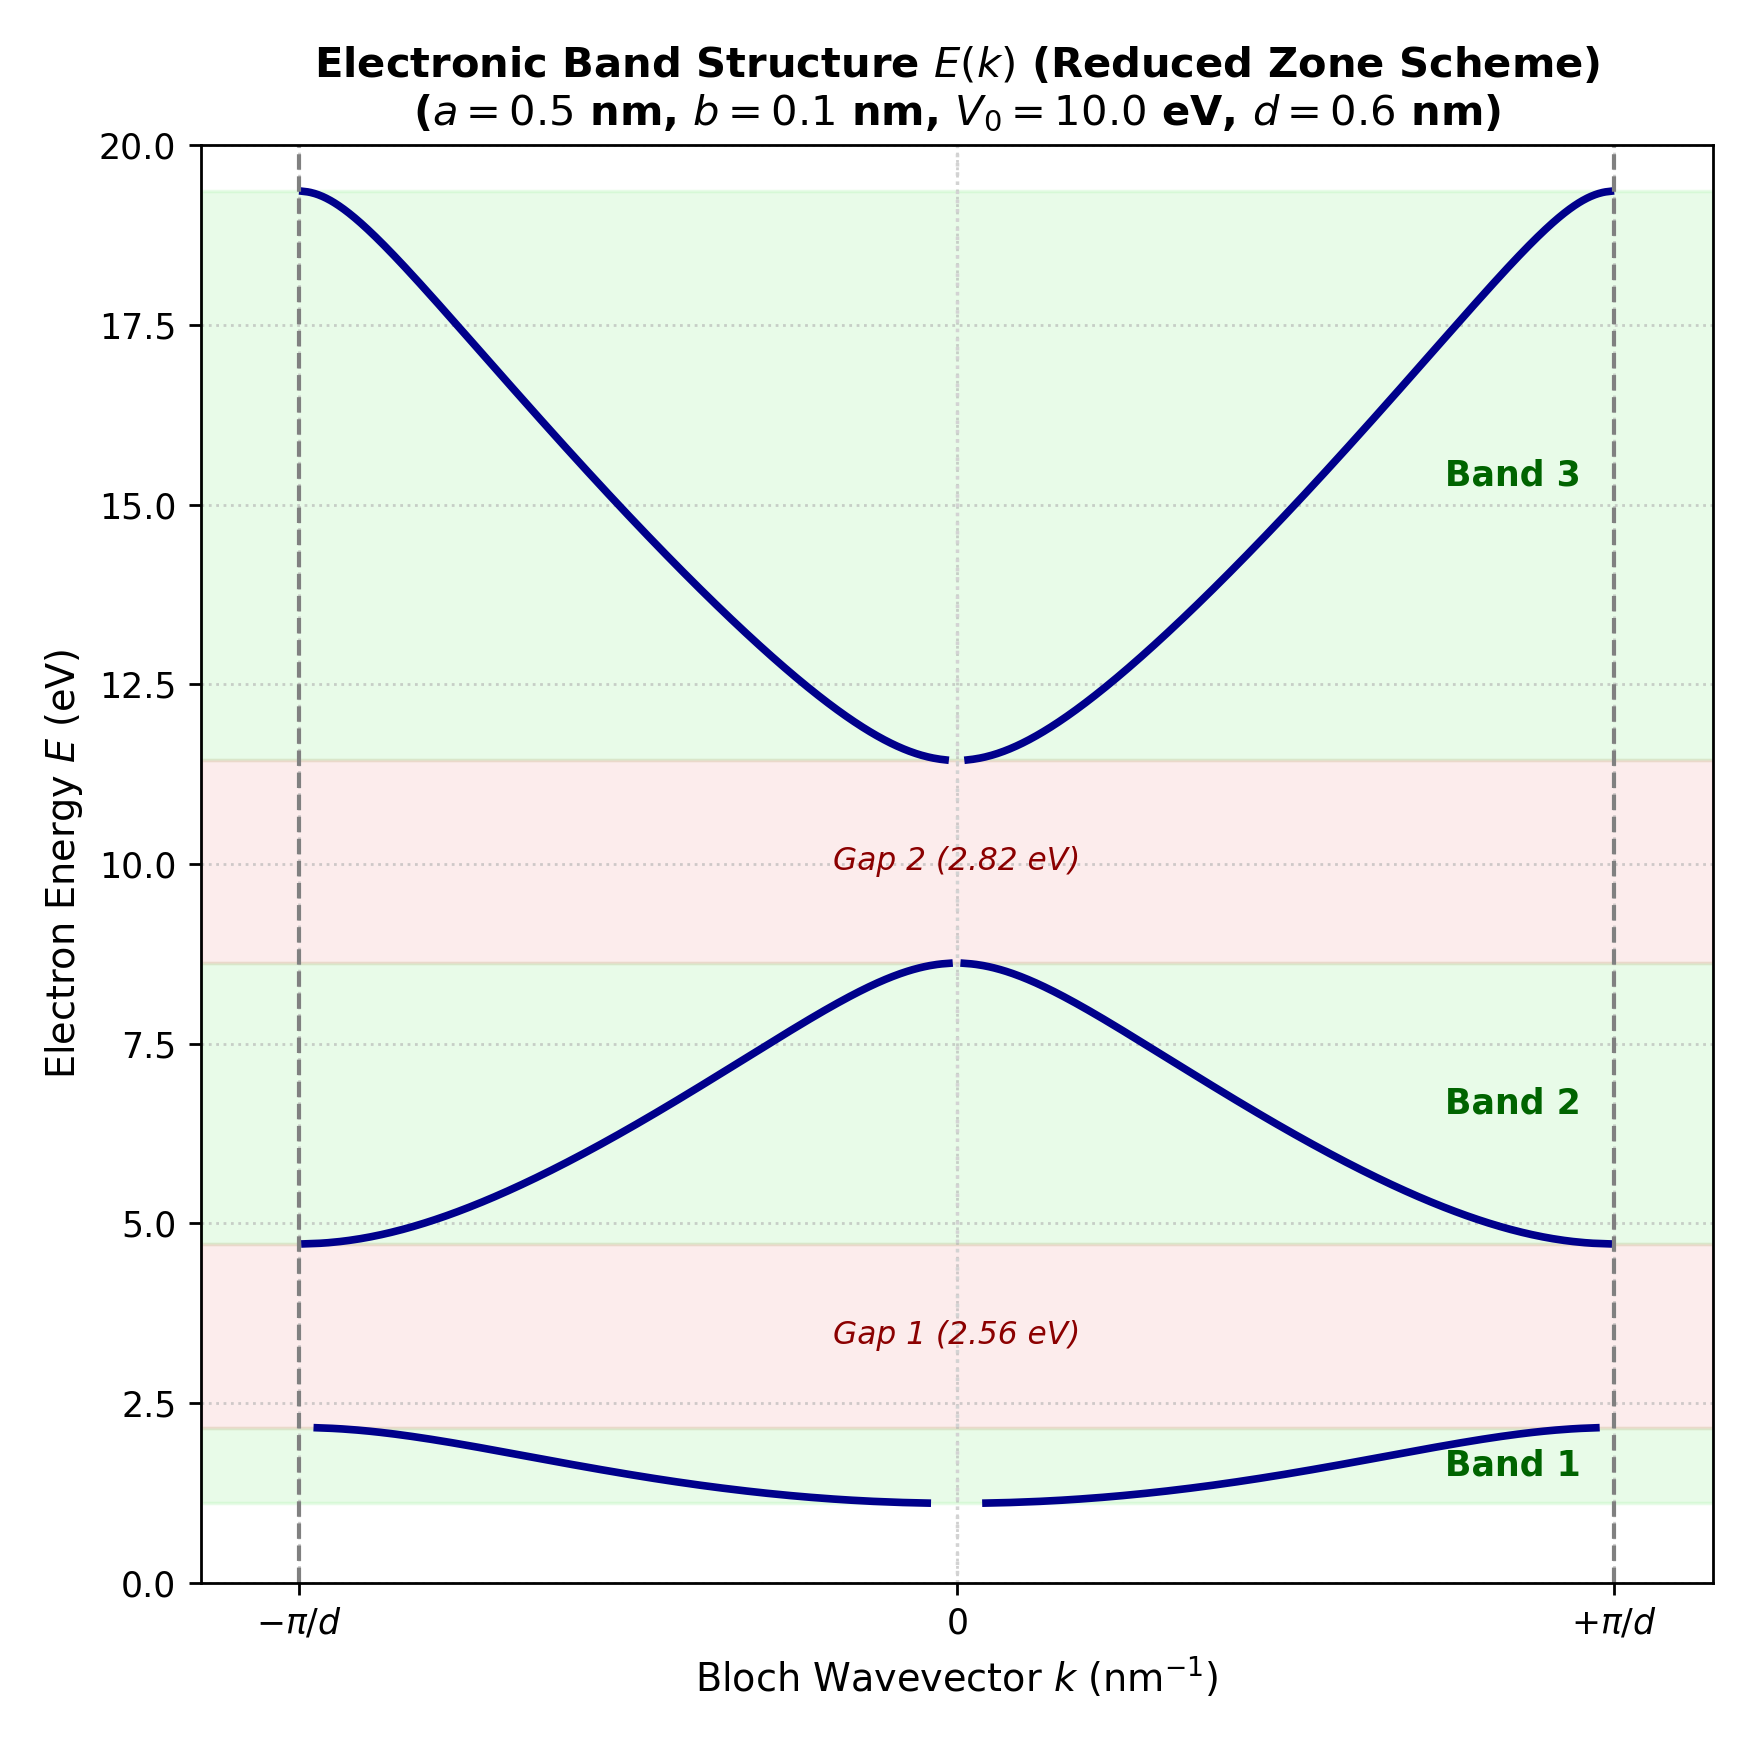
\includegraphics[width=0.48\textwidth]{figure3_ek_dispersion.png}
    \caption{\textbf{Reduced-zone $E(k)$ dispersion relation} across the first Brillouin zone $[-\pi/d, +\pi/d]$ for $a = 0.50\,\text{nm}, b = 0.10\,\text{nm}, V_0 = 10.0\,\text{eV}$. Shaded horizontal bands indicate allowed energy intervals; intervening white gaps denote forbidden states where $|f(E)| > 1$. Horizontal dashed line marks the barrier height $V_0 = 10\,\text{eV}$.}
    \label{fig:ek}
\end{figure}

\textbf{Comprehensive Physical Interpretation of the Band Structure:}
\begin{enumerate}\setlength{\itemsep}{1pt}\setlength{\parskip}{1pt}
    \item \textbf{Gap Opening at Zone Boundaries ($k = \pm\pi/d$):}
    At zone boundaries $k = \pm\pi/d$, de Broglie wavelength is $\lambda = 2d$, satisfying Bragg reflection. Incident and reflected waves superpose into two orthogonal standing waves: $\psi_+(x) \propto \cos(\pi x/d)$ (concentrated in wells, lower energy) and $\psi_-(x) \propto \sin(\pi x/d)$ (concentrated in barriers, higher energy). This electrostatic potential energy difference opens forbidden gaps (Gap 1: $2.556\,\text{eV}$; Gap 2: $2.821\,\text{eV}$).
    \item \textbf{Vanishing Group Velocity ($v_g = 0$):}
    The slope defines wavepacket group velocity $v_g = \frac{1}{\hbar}\frac{dE}{dk}$. At $k = 0$ and $k = \pm\pi/d$, $\frac{dE}{dk} = 0$, meaning electron group velocity strictly vanishes, forming stationary standing waves.
    \item \textbf{Effective Mass Curvature ($m^*$):}
    The effective mass is $m^* = \hbar^2\left(\frac{d^2E}{dk^2}\right)^{-1}$. Near band minima ($k \approx 0$), curvature is upward ($m^* > 0$, electron-like). Near band maxima ($k \approx \pm\pi/d$), curvature is downward ($m^* < 0$, giving rise to the \textit{hole} concept in semiconductors).
    \item \textbf{Bandwidth Widening at Higher Energies:}
    Band 1 ($E \ll V_0$) is narrow ($\Delta E_1 = 1.055\,\text{eV}$, tight-binding limit). Band 3 ($E > V_0$) is broad ($\Delta E_3 = 7.921\,\text{eV}$), approaching free-electron dispersion.
\end{enumerate}

\subsection{Parameter Sweep: Well Width \texorpdfstring{$a$}{a} \& Confinement Scaling (Question 6)}

To address Question 6, we numerically solved the TISE across varying well widths $a \in [0.20, 1.20]\,\text{nm}$ holding $b = 0.10\,\text{nm}$ and $V_0 = 10.0\,\text{eV}$ constant ($N = 4$ wells). The complete numerical eigenvalue evolution is compiled in Figure~\ref{fig:sweep} and quantified in Table~\ref{tab:sweep}.

\begin{figure}[H]
    \centering
    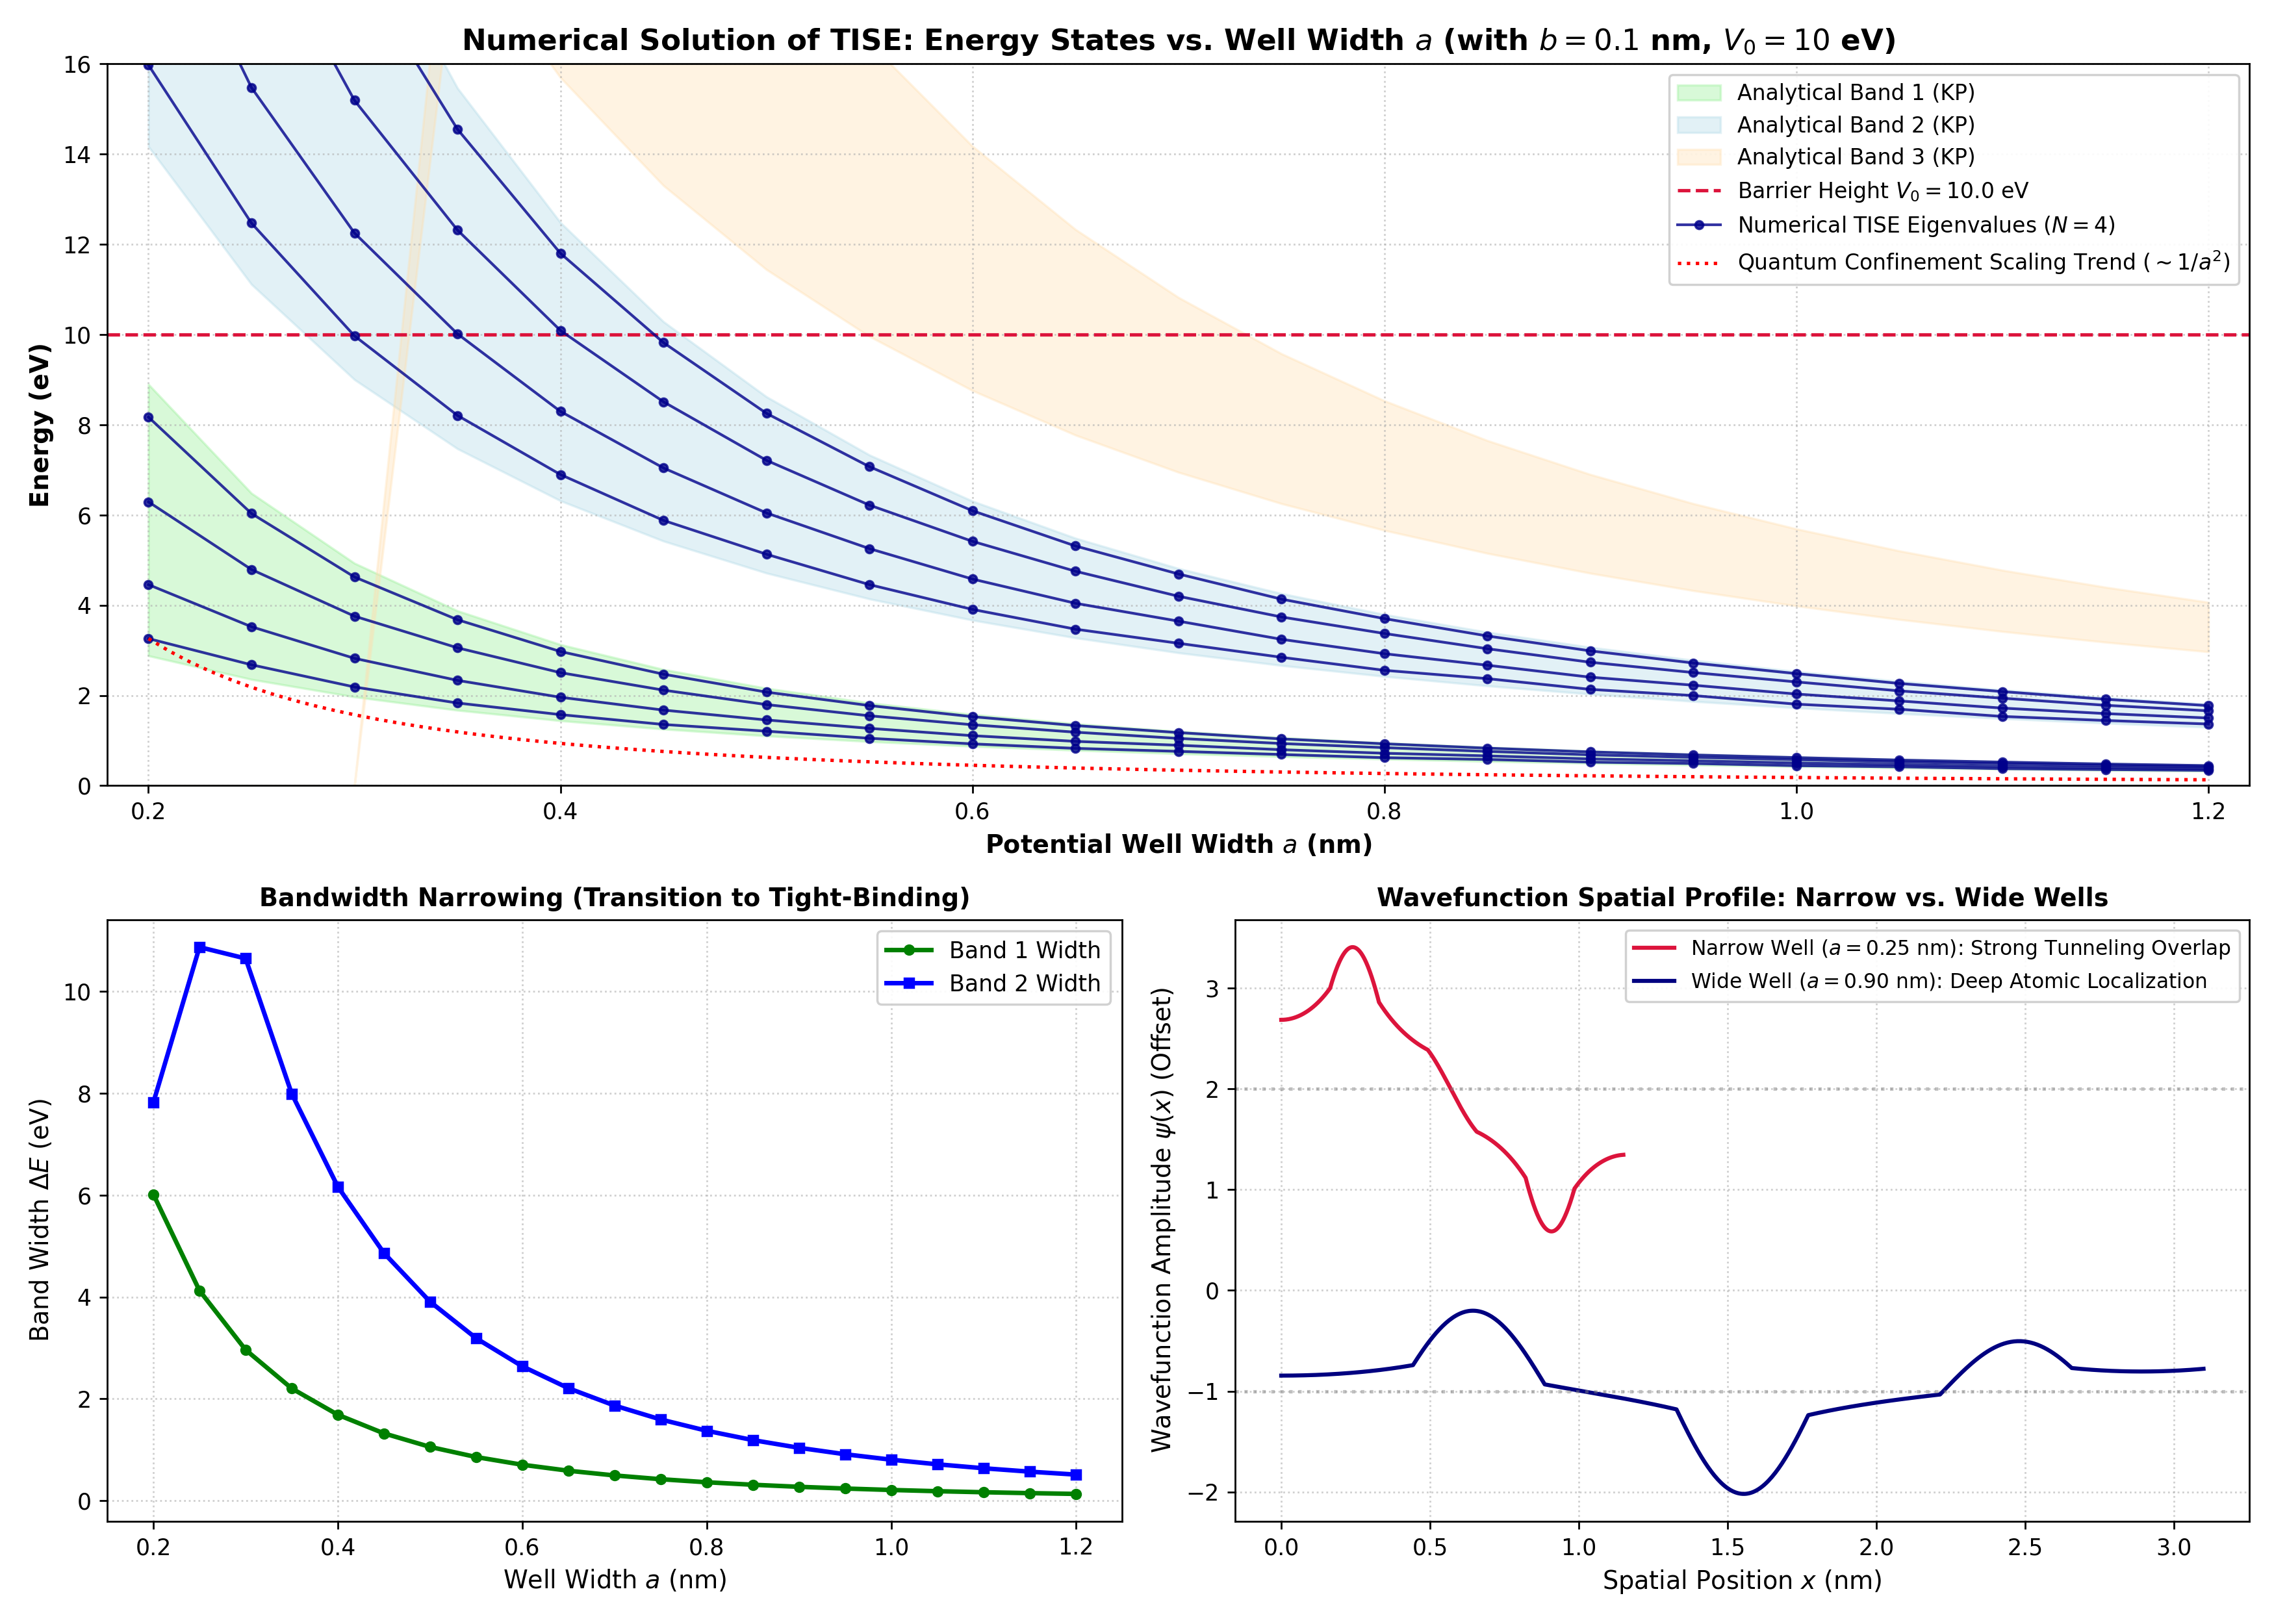
\includegraphics[width=0.78\textwidth]{figure4_parameter_sweep_a.png}
    \caption{\textbf{Numerical parameter sweep vs.\ well width $a$} ($b = 0.10\,\text{nm}$, $V_0 = 10.0\,\text{eV}$, $N = 4$ wells). \textbf{Top:} Discrete numerical eigenvalues (blue dots) clustering within analytical Kronig--Penney bands (shaded green); red dashed curve tracks ground-state confinement scaling. \textbf{Bottom-Left:} Band 1 width $\Delta E$ vs.\ $a$, showing dramatic compression into discrete atomic levels. \textbf{Bottom-Right:} Wavefunction comparison: strong inter-well tunneling leakage at $a = 0.25\,\text{nm}$ vs.\ tightly bound isolated states at $a = 0.90\,\text{nm}$.}
    \label{fig:sweep}
\end{figure}

\begin{table}[H]
\centering\footnotesize
\caption{Numerical finite-difference eigenvalues and Band 1 width $\Delta E$ as a function of well width $a$ ($N = 4$ wells).}
\label{tab:sweep}
\begin{tabular}{ccccccc}
\toprule
\textbf{$a$ (nm)} & \textbf{$E_1$ (eV)} & \textbf{$E_2$ (eV)} & \textbf{$E_3$ (eV)} & \textbf{$E_4$ (eV)} & \textbf{$\Delta E_1$ (eV)} & \textbf{Physical Regime} \\
\midrule
\textbf{0.20} & 3.2593 & 4.4555 & 6.2913 & 8.1698 & 4.9105 & Ultra-strong confinement, wide band \\
\textbf{0.40} & 1.5740 & 1.9586 & 2.5043 & 2.9726 & 1.3986 & Semiconductor superlattice \\
\textbf{0.60} & 0.9255 & 1.1074 & 1.3497 & 1.5282 & 0.6027 & Moderate confinement \\
\textbf{0.80} & 0.6196 & 0.7175 & 0.8421 & 0.9271 & 0.3075 & Tight-binding transition \\
\textbf{1.00} & 0.4426 & 0.5017 & 0.5744 & 0.6214 & 0.1788 & Quasi-discrete atomic states \\
\textbf{1.20} & 0.3380 & 0.3725 & 0.4145 & 0.4437 & 0.1057 & Isolated atomic limit (near-degeneracy) \\
\bottomrule
\end{tabular}
\end{table}

\textbf{Physical Mechanisms Driving the Parameter Evolution:}
\begin{enumerate}\setlength{\itemsep}{1pt}\setlength{\parskip}{1pt}
    \item \textbf{Quantum Confinement Effect ($E \propto 1/a^2$):}
    Kinetic energy scales as $\langle T \rangle \sim \frac{\pi^2\hbar^2}{2m_e a^2}$. As $a$ expands, the confinement box widens, shifting all eigenvalues downward along the $1/a^2$ envelope (red dashed curve in Figure~\ref{fig:sweep}).
    \item \textbf{Proliferation of Bound States:}
    At $a = 0.20\,\text{nm}$, the well holds only 1 band below $V_0 = 10\,\text{eV}$. Expanding $a$ to $1.20\,\text{nm}$ accommodates 4 allowed bands below $V_0$.
    \item \textbf{Bandwidth Compression into Tight-Binding Limit:}
    Band 1 width collapses from $4.91\,\text{eV}$ down to $0.11\,\text{eV}$ (45-fold narrowing). For small $a$, states sit near the barrier top ($E \sim V_0$), making $\beta = \sqrt{(V_0-E)/\gamma}$ small, yielding strong tunneling overlap. For large $a$, states sink deep into wells ($E \ll V_0$), making $\beta$ large and tunneling negligible. Bands compress into $N$-fold degenerate atomic levels.
    \item \textbf{Cluster Splitting ($N$ States per Band):}
    For $N = 4$, exactly 4 eigenvalues cluster inside each band, verifying that an $N$-cell crystal splits each atomic level into $N$ distinct quantum states.
\end{enumerate}

\section{Code Architecture \& Implementation Details (Question 7)}

The codebase is organized into modular Python files adhering to single-responsibility design, summarized in Table~\ref{tab:code}.

\begin{table}[H]
\centering\footnotesize
\caption{Codebase architecture, module responsibilities, and computational functions.}
\label{tab:code}
\begin{tabular}{p{3.8cm}p{3.0cm}p{9.4cm}}
\toprule
\textbf{File} & \textbf{Role / Framework} & \textbf{Key Responsibilities \& Core Algorithms} \\
\midrule
\texttt{kp\_engine.py} & Core Physics Engine & Dispersion $f(E)$ evaluation (Eqs.~\ref{eq:kp_below},~\ref{eq:kp_above}), automated band edge root-finding via \texttt{scipy.optimize.brentq}, unimodular Transfer Matrix Method (TMM) wavefunction construction, and tridiagonal matrix TISE solver via \texttt{eigh\_tridiagonal}. \\
\texttt{app.py} & Interactive GUI (Streamlit) & Reactive scientific dashboard with 5 physical sliders ($N, E, a, b, V_0$), live allowed/forbidden status badges, presets, and 4 dedicated visualization tabs. \\
\texttt{numerical\_analysis.py} & Parameter Sweep Solver & Standalone numerical pipeline for Question 6: sweeps well width $a \in [0.2, 1.2]\,\text{nm}$, extracts eigenvalues, computes bandwidth narrowing, and generates Figure 4. \\
\texttt{plot\_generator.py} & Visualization Pipeline & Generates publication-quality figures: Figure 1 (allowed state), Figure 2 (forbidden gap), and Figure 3 ($E(k)$ dispersion relation) with exact annotations. \\
\texttt{demo\_runner.py} & Automated Test Suite & Master verification CLI script validating all algorithms against analytical benchmarks without requiring GUI interaction. \\
\bottomrule
\end{tabular}
\end{table}

\textbf{Numerical Robustness \& Execution Instructions:}
All computations strictly operate in nanoscale units ($\text{eV}, \text{nm}, m_e$) using $\gamma = \hbar^2/(2m_e) = 0.0761996\,\text{eV}\cdot\text{nm}^2$, avoiding floating-point overflows ($\sim 10^{-68}$) inherent to raw SI calculations. Transfer matrices are enforced unimodular ($\det\mathbf{M} = 1$), ensuring energy conservation and stability.
\begin{lstlisting}[language=bash]
# Install prerequisites -> Launch interactive GUI -> Run automated test suite
pip install numpy scipy matplotlib streamlit
streamlit run app.py
python3 demo_runner.py && python3 numerical_analysis.py
\end{lstlisting}

\section{Conclusion \& Summary of Findings}
This project delivered a complete, interactive, and academically rigorous study of the Kronig--Penney model:
\begin{itemize}\setlength{\itemsep}{0pt}\setlength{\parskip}{0.5pt}
    \item \textbf{Question 1 (Theory):} Derived the secular master equation from boundary continuity; explained band formation and Bragg reflection.
    \item \textbf{Question 2 (Interface):} Built a reactive Streamlit application with 5 adjustable controls, presets, and live diagnostics.
    \item \textbf{Question 3 (Dispersion \& Bands):} Computed exact energy bands and gaps via Brent's method; mapped reduced-zone $E(k)$ diagrams.
    \item \textbf{Question 4 (Wavefunction):} Visualized continuous $\psi(x)$ across multi-well superlattices, verifying smooth interface matching.
    \item \textbf{Question 5 (Probability Density):} Evaluated $|\psi(x)|^2$, proving charge localization at nuclei and contrasting propagating vs.\ evanescent states.
    \item \textbf{Question 6 (Numerical TISE \& Parameter Sweep):} Solved the TISE numerically via finite differences; parameter sweeps vs.\ $a$ proved quantum confinement ($E \propto 1/a^2$), bound state proliferation, and bandwidth collapse into the tight-binding limit.
    \item \textbf{Question 7 (Code \& Interpretations):} Provided clean, modular, fully-commented Python scripts with reproducible execution pipelines.
\end{itemize}

\begin{thebibliography}{6}
\bibitem{kronig1931} Kronig, R. de L., \& Penney, W. G. (1931). \textit{A Quantum Mechanics of Electrons in Crystal Lattices}. Proceedings of the Royal Society of London. Series A, 130(814), 499--513.
\bibitem{kittel2004} Kittel, C. (2004). \textit{Introduction to Solid State Physics} (8th ed.). John Wiley \& Sons. Chapters 7 \& 8.
\bibitem{ashcroft1976} Ashcroft, N. W., \& Mermin, N. D. (1976). \textit{Solid State Physics}. Saunders College Publishing. Chapters 8 \& 9.
\bibitem{griffiths2018} Griffiths, D. J., \& Schroeter, D. F. (2018). \textit{Introduction to Quantum Mechanics} (3rd ed.). Cambridge University Press. Section 5.3.
\bibitem{davies1998} Davies, J. H. (1998). \textit{The Physics of Low-Dimensional Semiconductors: An Introduction}. Cambridge University Press.
\bibitem{harris2020} Harris, C. R., et al. (2020). \textit{Array programming with NumPy}. Nature, 585(7825), 357--362.
\end{thebibliography}

\end{document}
